% Trading-bot dissertation. Compiles with a standard TeX distribution:
%   pdflatex thesis.tex   (run twice for the table of contents / refs)
% or upload to Overleaf (thesis.tex + the figures/ folder).
\documentclass[11pt,a4paper]{article}

\usepackage[utf8]{inputenc}
\usepackage[T1]{fontenc}
\usepackage{lmodern}
\usepackage[a4paper,margin=1in]{geometry}
\usepackage{booktabs}
\usepackage{graphicx}
\usepackage{array}
\usepackage{amsmath}
\usepackage{xcolor}
\usepackage{caption}
\usepackage{enumitem}
\usepackage{parskip}
\usepackage[hidelinks]{hyperref}

\captionsetup{font=small,labelfont=bf}
\newcommand{\tbot}[1]{\texttt{#1}}

\title{\textbf{Building a Rules-Based Algorithmic Trading System,\\ and an Empirical Test of Whether Simple Technical\\ Strategies Have a Tradeable Edge}}
\author{Masimba}
\date{29 May 2026}

\begin{document}
\maketitle

\begin{center}
\small
Repository: \texttt{github.com/MasimbaTakudzwa/trading-strategy-edge-study} \quad$\vert$\quad
Stack: Python 3.12 $\cdot$ cTrader Open API (FP Markets) $\cdot$ TimescaleDB $\cdot$ vectorbt
\end{center}

\begin{abstract}
\noindent This report documents the design, implementation, and empirical evaluation of a production-grade algorithmic trading bot built from scratch in Python. The system spans the full pipeline --- market-data acquisition, persistence, strategy signal generation, vectorised backtesting, volatility-based risk management, an order-management system (OMS) with a broker adapter, a live paper-trading engine, and observability tooling --- integrated against a real broker (FP Markets) via the cTrader Open API, with defence-in-depth safeguards to prevent unintended live trading.

The engineering objective was met in full: a safe, tested (114 automated tests), broker-integrated system that places correctly-sized, risk-checked, idempotent orders on a demo account. The \textbf{trading} objective --- a durable, profitable edge from simple technical rules --- was \textbf{not} met, and this report argues that this is the empirically expected outcome. Across \textbf{six backtests} spanning two instruments (gold, EUR/USD), two strategy families (trend-following, mean-reversion), two timeframes (hourly, daily), and horizons up to \textbf{22 years}, no configuration produced a risk-adjusted edge that survives realistic costs; in every clean comparison, passive buy-and-hold matched or beat the active strategy. The most striking result: over 22 years a trend strategy on gold returned \textbf{+28.6\%} while simply holding gold returned \textbf{+983.6\%}. We present the engineering, the methodology, the full results, an honest discussion of \emph{why} no edge was found, the threats to validity, and recommended future work. The contribution is twofold: a reusable trading-system architecture, and a rigorously-established negative result of the kind retail practitioners rarely reach before committing capital.
\end{abstract}

\tableofcontents
\newpage

\section{Introduction and Objectives}
The goal was to build --- not buy or wire together --- a complete algorithmic trading bot for a retail-scale account, and to use it to answer a concrete empirical question:
\begin{quote}
\emph{Can a disciplined, rules-based technical strategy, executed by a well-engineered bot, produce a durable edge on liquid markets after realistic costs?}
\end{quote}
Two distinct objectives followed:
\begin{itemize}[leftmargin=1.4em]
  \item \textbf{Engineering objective.} Build a safe, testable, broker-integrated system covering the entire lifecycle: data $\to$ signals $\to$ backtest $\to$ risk $\to$ execution $\to$ live loop $\to$ monitoring.
  \item \textbf{Trading objective.} Identify a strategy/instrument with a positive, repeatable, risk-adjusted edge worth trading with real money.
\end{itemize}
A core principle governed the project: \textbf{the bot must never place a live order until its behaviour has been verified.} This shaped a defence-in-depth safety design (Section~\ref{sec:safety}) and a ``validation-first'' workflow --- build, backtest, then paper-trade on a demo account, deferring any live capital.

\section{Constraints and Context}
The problem was shaped by the operator's real-world constraints, which materially narrowed the design space.

\begin{table}[ht]\centering
\caption{Operating constraints and their implications.}
\begin{tabular}{@{}p{5.3cm}p{8.2cm}@{}}
\toprule
\textbf{Constraint} & \textbf{Implication} \\
\midrule
Operator located in \textbf{Zimbabwe} & Most major brokers (and all US-based ones) do not accept clients; broker choice was severely restricted. \\
\textbf{Free API} required & Ruled out paid vendors; drove the choice of the cTrader Open API. \\
\textbf{Sub-\$1{,}000} account & Minimum contract sizes become a hard constraint (Section~\ref{sec:minsize}). \\
\textbf{No crypto} (purely speculative) & Excluded the most API-accessible retail market. \\
\textbf{Stability preferred} & Favoured simple, well-understood technical strategies. \\
\bottomrule
\end{tabular}
\end{table}

\noindent\textbf{Broker selection.} After surveying options, \textbf{FP Markets} (cTrader Raw demo account) was selected as the only cTrader broker found to accept Zimbabwean clients while exposing a free, programmatic API.

\noindent\textbf{Market pivot.} The project began on FX majors but pivoted mid-way: \emph{``currency trading is way too hard to predict and is de-railed by government decisions.''} Focus moved to commodities (precious metals) and indices. EUR/USD is retained as a \textbf{control instrument} --- not a live target, but (a)~the only instrument whose minimum size fits a \$1{,}000 account, and (b)~as a non-appreciating currency pair it provides a \emph{flat} buy-and-hold benchmark, isolating pure strategy skill from asset drift.

\section{System Architecture}
\subsection{Pipeline}
The system is a one-directional pipeline of small, independently-testable components communicating through well-defined interfaces (Python \tbot{Protocol}s). Strategies never import a broker; the broker is swappable behind an adapter. The flow is:
\begin{center}
\tbot{cTrader API} $\to$ \tbot{Fetcher/DB} $\to$ \tbot{Strategy} $\to$ \tbot{Risk Gate} $\to$ \tbot{OMS} $\to$ \tbot{Broker (demo)},
\end{center}
with the \tbot{Backtest} engine drawing from \tbot{Strategy}, and the \tbot{Observability} commands reading from the OMS's persisted runs/orders/trades.

\begin{table}[ht]\centering
\caption{Component summary.}
\begin{tabular}{@{}llp{7.2cm}@{}}
\toprule
\textbf{Layer} & \textbf{Module} & \textbf{Responsibility} \\
\midrule
Data & \tbot{data/ctrader\_fetcher} & Paginated candle download; idempotent upsert into TimescaleDB; DB$\to$DataFrame loader. \\
Protocol & \tbot{data/ctrader\_protocol} & Sync facade over the Twisted SDK (via \tbot{crochet}); auth; send/recv; retry. \\
Strategy & \tbot{strategies/*} & Pure, look-ahead-safe signal generators. \\
Backtest & \tbot{backtest/runner} & vectorbt portfolio simulation with a realistic cost model. \\
Risk & \tbot{risk/*} & ATR volatility sizing; per-trade/daily/exposure limits; kill switch; live-trading guards. \\
Execution & \tbot{execution/*} & Broker \tbot{Protocol}; unit$\leftrightarrow$volume conversion + min-size guard; cTrader adapter. \\
OMS & \tbot{oms/*} & Sizing$\to$risk-check$\to$idempotent placement; run persistence; live loop; reconciliation; reporting. \\
Interface & \tbot{cli} & The \tbot{tbot} CLI: \tbot{fetch}, \tbot{backtest}, \tbot{paper}, \tbot{status}, \tbot{reconcile}, \tbot{report}, \tbot{safety}. \\
\bottomrule
\end{tabular}
\end{table}

\subsection{Defence-in-depth safety}\label{sec:safety}
Because the prime directive was ``never trade live until verified,'' live order placement is gated by \textbf{three independent layers}, all of which must pass:
\begin{enumerate}[leftmargin=1.6em]
  \item \textbf{Host isolation} --- configuration selects the demo vs.\ live endpoint.
  \item \textbf{\tbot{ALLOW\_LIVE\_TRADING} switch} --- defaults to \tbot{false}; live orders are impossible unless explicitly enabled.
  \item \textbf{Account \tbot{isLive} check} --- the adapter verifies the authenticated account's status before any order.
\end{enumerate}
The \tbot{paper} command additionally hard-requires \tbot{CTRADER\_ENV=demo}. Position-reducing actions (closes, the kill switch) are intentionally \emph{not} gated, so the bot can always flatten risk. Throughout all testing, the live account was never touched.

\section{The cTrader API Implementation}
The cTrader Open API is a \textbf{protobuf-over-TLS} protocol (port 5035) delivered through an official SDK built on the \textbf{Twisted} asynchronous reactor. Integrating it into an otherwise synchronous codebase was the hardest single piece of engineering.

\noindent\textbf{Sync facade via crochet.} The Twisted reactor runs in a background thread (\tbot{crochet}); a thin facade exposes blocking \tbot{connect()}/\tbot{send()} methods, keeping Twisted out of strategy, risk, and CLI code entirely.

\noindent\textbf{Authentication.} A three-step ceremony: TLS connect $\to$ application auth (app credentials) $\to$ account auth (account id + OAuth access token). A separate OAuth 2.0 authorization-code flow (\tbot{tbot ctrader login}, a local callback server) obtains and refreshes tokens.

\begin{table}[ht]\centering
\caption{cTrader encoding facts (verified against live specs; a frequent source of bugs).}
\begin{tabular}{@{}lp{8.5cm}@{}}
\toprule
\textbf{Quantity} & \textbf{Rule} \\
\midrule
Price & scaled by $\div 100000$ uniformly \\
Order volume & $\text{volume} = \text{units} \times 100$ (1{,}000 units of EUR/USD $=$ volume 100{,}000) \\
Money & scaled by $\div 10^{\text{moneyDigits}}$ \\
Responses & delivered as \tbot{ProtoMessage} envelopes; must be extracted before use \\
\bottomrule
\end{tabular}
\end{table}

\noindent\textbf{Resilience.} \tbot{send()} is wrapped in a \tbot{tenacity} retry that retries \emph{transient} transport failures (connection drops, timeouts) with exponential backoff, while letting \emph{logical} API errors propagate immediately. Re-sending is safe because every order carries an idempotency key (Section~\ref{sec:oms}). This retry was hardened after a real failure (Section~\ref{sec:forward}).

\section{Strategy Design}
Two complementary, deliberately simple strategies were implemented. Both are \textbf{pure functions} of price (no I/O), making them identical in backtest, paper, and live --- and both are \textbf{look-ahead-safe}: every indicator at bar $t$ is computed only from bars $t-1$ and earlier, then compared to bar $t$'s close.

\noindent\textbf{Donchian channel breakout (trend-following).} A stripped-down Turtle system. \emph{Long} when close breaks above the highest high of the prior $N$ bars; \emph{exit} when it falls below the lowest low of the prior $M$ bars (shorts mirror). Tested with the classic long-term parameters $N=55$, $M=20$.

\noindent\textbf{Bollinger-band mean-reversion.} Bets that price snaps back to its mean. \emph{Long} when close falls below the lower band ($\text{mean} - k\sigma$ over $N$ bars); \emph{exit} at the mean (shorts mirror). Tested at $N=20$, $k=2.0$. Rationale: FX majors \emph{range} rather than trend in the modern regime. Documented failure mode: a strong trend that does not revert.

\section{Risk Management}
\subsection{Volatility position sizing}
Every trade risks a constant fraction of equity. Given a stop distance and the money value of a one-point move, the size that risks exactly $\text{equity} \times \text{risk fraction}$ is:
\[ \text{units} \;=\; \frac{\text{equity} \times \text{risk fraction}}{\text{stop distance} \times \text{value per point}}. \]
The stop distance is volatility-scaled: $\text{stop} = \text{ATR}(14) \times 2$. Default per-trade risk is \textbf{0.5\%}.

\subsection{Limits and the kill switch}
The risk gate enforces, in order: a \textbf{kill switch} (halt on daily drawdown breaching 2\%), a \textbf{max-open-positions} cap, a \textbf{leverage} cap, and a mandatory \textbf{stop-loss-present} check. Any failure short-circuits before the order reaches the broker.

\subsection{The small-account minimum-size wall}\label{sec:minsize}
A pivotal finding. At 0.5\% risk, the per-trade budget on a \$1{,}000 account is \textbf{\$5}. The smallest tradeable size of many instruments already risks far more.

\begin{table}[ht]\centering
\caption{Minimum-size risk vs.\ a \$5 per-trade budget on a \$1{,}000 account.}
\begin{tabular}{@{}llrrl@{}}
\toprule
\textbf{Instrument} & \textbf{Min size} & \textbf{Risk} & \textbf{\% of \$1{,}000} & \textbf{Fits?} \\
\midrule
EUR/USD & 1{,}000 units (micro-lot) & $\approx\$5$ & 0.5\% & Yes \\
Gold (XAUUSD) & 1 oz & $\approx\$150$ & 15\% & No \\
Equity index & 1 contract & $\approx\$140$ & 14\% & No \\
\bottomrule
\end{tabular}
\end{table}

\noindent The \tbot{fit\_order\_size} guard \textbf{refuses} any order whose minimum size exceeds the budget. Consequently, on a \$1{,}000 account only FX micro-lots size safely; gold needs roughly \textbf{\$30{,}000} before its minimum fits. This is why EUR/USD is the only instrument used for \emph{live/paper} sizing --- though backtesting (which is size-independent) was run freely on gold.

\section{Execution and the Order-Management System}\label{sec:oms}
The OMS is the single choke point every order passes through. \tbot{open\_position()} executes, in strict order:
\begin{enumerate}[leftmargin=1.6em,itemsep=0pt]
  \item ATR-size the position (constant money-at-risk);
  \item fit to broker volume constraints $+$ the min-size guard;
  \item derive the stop price from the ATR stop distance;
  \item mint a \textbf{deterministic, idempotent \tbot{client\_order\_id}} $=$ SHA-1 of $(\text{run}, \text{instrument}, \text{bar}, \text{side})$;
  \item run the risk gate;
  \item place via the broker adapter.
\end{enumerate}
Any failed gate short-circuits with a reason; the order never reaches the broker. The idempotency key means re-processing the same bar --- e.g.\ after a restart --- cannot double-submit. Trades are recorded on entry and settled (with realised P\&L) on close, powering the reporting layer.

\section{Backtesting Methodology}
\textbf{Engine.} vectorbt's vectorised (NumPy/Numba) portfolio simulator --- fast enough to replay decades of history in well under a second of compute.

\begin{table}[ht]\centering
\caption{Cost model (conservative; approximating an FP Markets cTrader Raw account).}
\begin{tabular}{@{}lll@{}}
\toprule
\textbf{Component} & \textbf{Value} & \textbf{Basis} \\
\midrule
Commission (\tbot{fees}) & 0.00003 / side & $\approx\$3$ per 100k-notional lot \\
Spread/slippage & 0.00002 / side & $\approx 0.1$-pip raw EUR/USD spread $+$ buffer \\
\bottomrule
\end{tabular}
\end{table}

\noindent\textbf{Benchmark.} Every run reports buy-and-hold of the same instrument over the same window --- the honest hurdle an active strategy must beat. \textbf{Data:} hourly (H1) history reached back to 2018; daily (D1) history reached back to late 2003 ($\sim$22 years), spanning the 2008 crisis, the 2011 gold peak, the 2013 crash, 2020, and the 2022 shock.

\begin{table}[ht]\centering
\caption{Measured backtest performance (steady-state, after JIT warm-up).}
\begin{tabular}{@{}lrrr@{}}
\toprule
\textbf{Dataset} & \textbf{Bars} & \textbf{Signal calc} & \textbf{vectorbt sim} \\
\midrule
$\sim$5 yr H1 FX & 30{,}000 & 2 ms & 0.36 s \\
$\sim$3.5 yr M15 FX & 120{,}000 & 8 ms & 1.5 s \\
$\sim$1.5 yr M1 FX & 500{,}000 & 33 ms & 6.5 s \\
\bottomrule
\end{tabular}
\end{table}

\noindent This speed is the entire argument for backtesting before forward-testing: 22 years of daily history replays in a fraction of a second, versus a real-time paper test that produced \emph{zero} trades overnight (Section~\ref{sec:forward}).

\section{Results}
\subsection{The scorecard}
All six backtests, \$1{,}000 initial capital, conservative costs applied. (PF $=$ profit factor; a tradeable strategy typically wants Sharpe $\ge 1.0$ and PF $\ge 1.3$.)

\begin{table}[ht]\centering
\caption{Full backtest scorecard.}
\resizebox{\textwidth}{!}{%
\begin{tabular}{@{}llllrrrrrrr@{}}
\toprule
\textbf{Instrument} & \textbf{TF} & \textbf{Strategy} & \textbf{Window} & \textbf{Return} & \textbf{Buy \& Hold} & \textbf{Max DD} & \textbf{Sharpe} & \textbf{Win \%} & \textbf{Trades} & \textbf{PF} \\
\midrule
Gold & D1 & Donchian 55/20 & 2004--2026 & 28.55\% & 983.61\% & 48.40\% & 0.18 & 38.0\% & 79 & 1.17 \\
Gold & H1 & Donchian 55/20 & 2018--2026 & 25.96\% & 244.46\% & 31.97\% & 0.33 & 39.4\% & 639 & 1.08 \\
EUR/USD & H1 & Donchian 55/20 & 2018--2026 & $-$11.25\% & $-$3.13\% & 25.80\% & $-$0.24 & 39.2\% & 711 & 0.93 \\
EUR/USD & H1 & Bollinger 20/2 & 2018--2026 & 5.89\% & $-$3.13\% & 11.67\% & 0.17 & 63.2\% & 2{,}278 & 1.02 \\
EUR/USD & D1 & Donchian 55/20 & 2004--2026 & $-$12.68\% & $-$7.45\% & 26.19\% & $-$0.06 & 32.2\% & 87 & 0.88 \\
EUR/USD & D1 & Bollinger 20/2 & 2004--2026 & $-$3.65\% & $-$7.45\% & 34.66\% & 0.01 & 64.6\% & 244 & 0.98 \\
\bottomrule
\end{tabular}}
\end{table}

\vspace{-0.4em}
\noindent\emph{Columns omitted for width: Sortino (0.25, 0.47, $-$0.34, 0.24, $-$0.09, 0.02) and bar counts (5{,}723 / 49{,}305 / 52{,}302 / 52{,}302 / 6{,}142 / 6{,}142).}

\subsection{Return vs.\ buy-and-hold}
\begin{figure}[ht]\centering
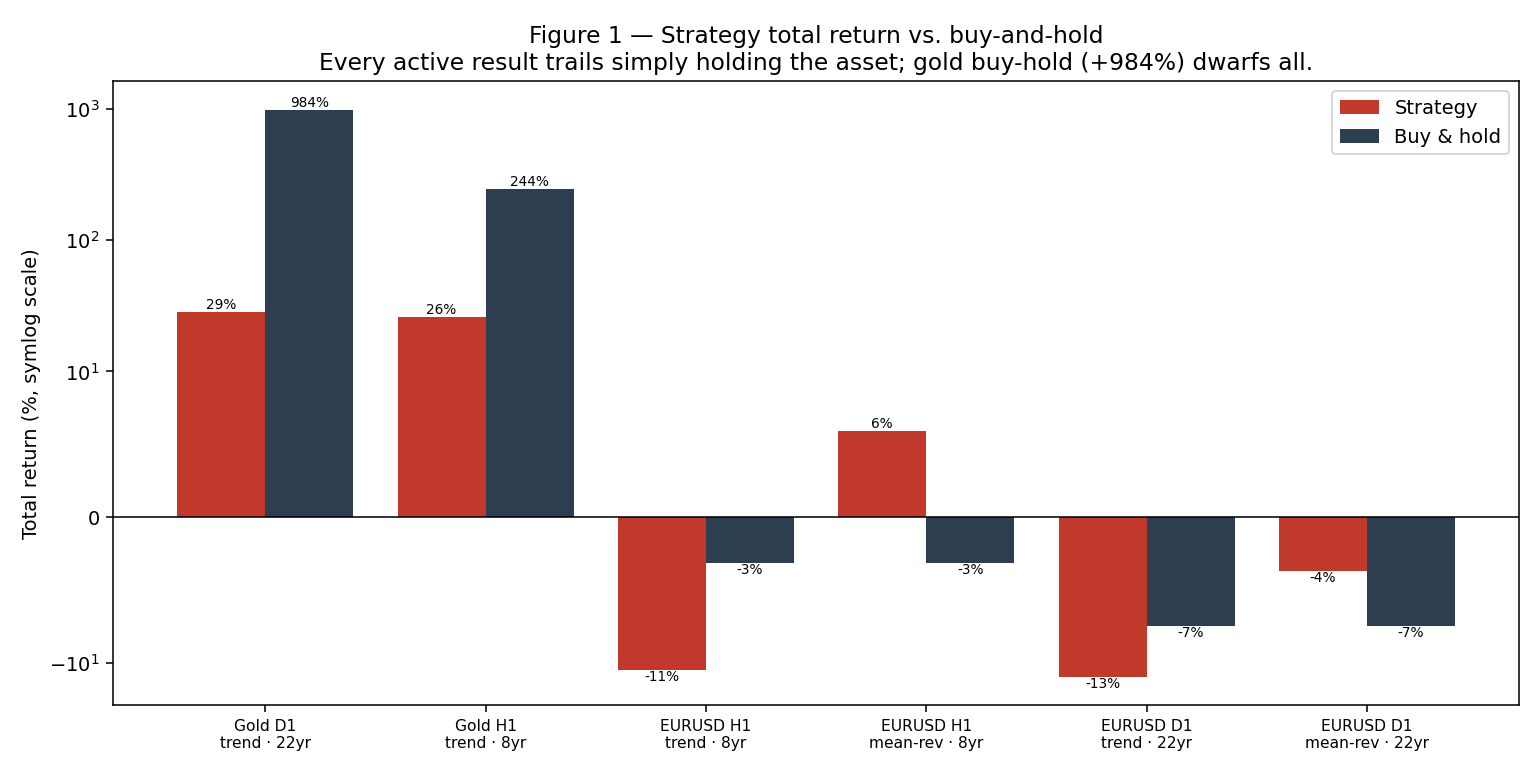
\includegraphics[width=\linewidth]{figures/fig1_return_vs_benchmark.png}
\caption{Strategy total return vs.\ buy-and-hold. Every active result trails simply holding the asset; gold's buy-and-hold (+984\%) dwarfs the +28.6\% the trend strategy extracted --- the active system captured roughly 3\% of the available return.}
\end{figure}

\subsection{Risk-adjusted quality}
\begin{figure}[ht]\centering
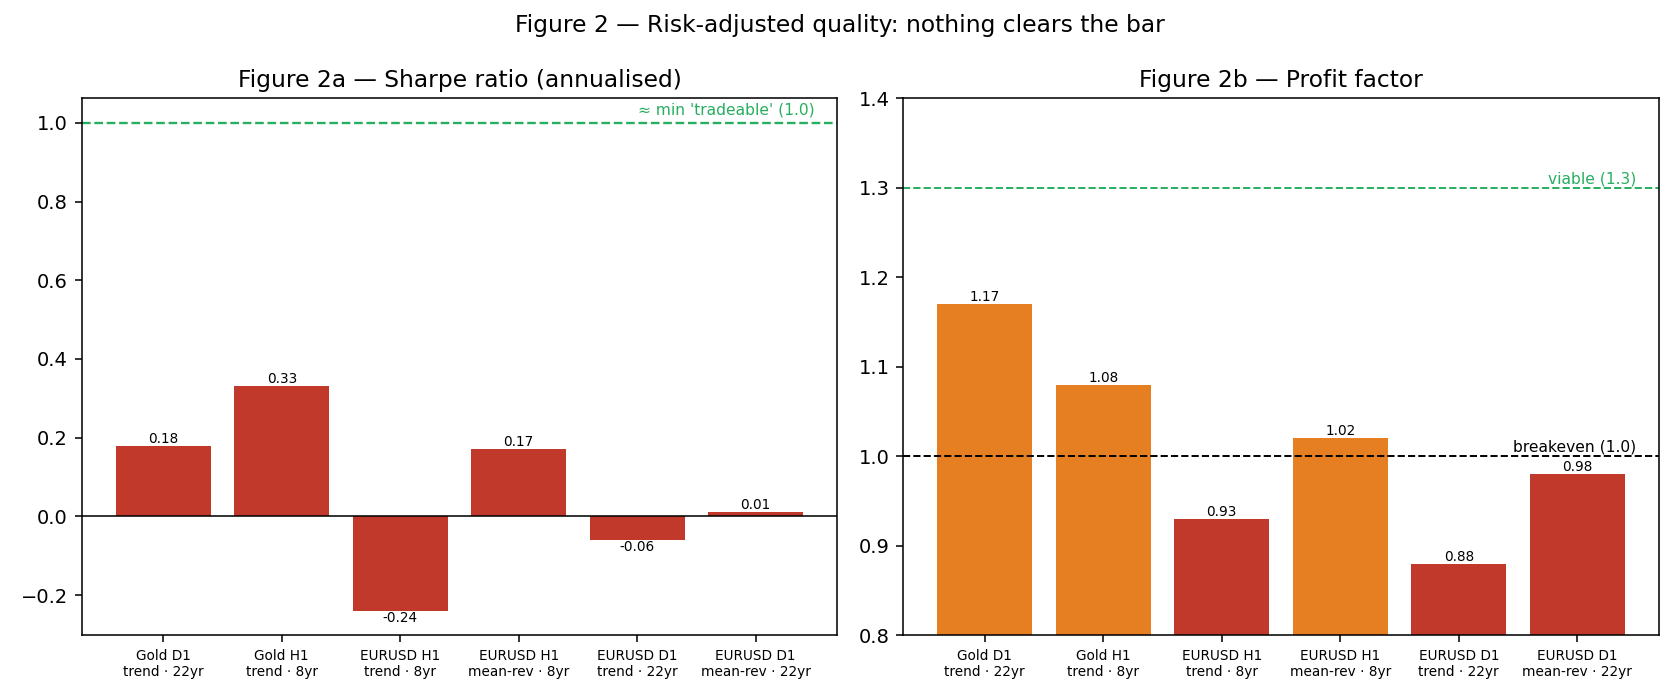
\includegraphics[width=\linewidth]{figures/fig2_risk_metrics.png}
\caption{Sharpe ratio and profit factor across all tests. No test reaches a Sharpe of 1.0 (peak 0.33); none reaches a profit factor of 1.3 (peak 1.17); three are below the 1.0 breakeven line. The best profit factor (gold trend, 1.17) comes from only 79 trades --- the least cost-sensitive figure available --- and is still not viable.}
\end{figure}

\subsection{Equity curves (the 22-year daily tests)}
\begin{figure}[ht]\centering
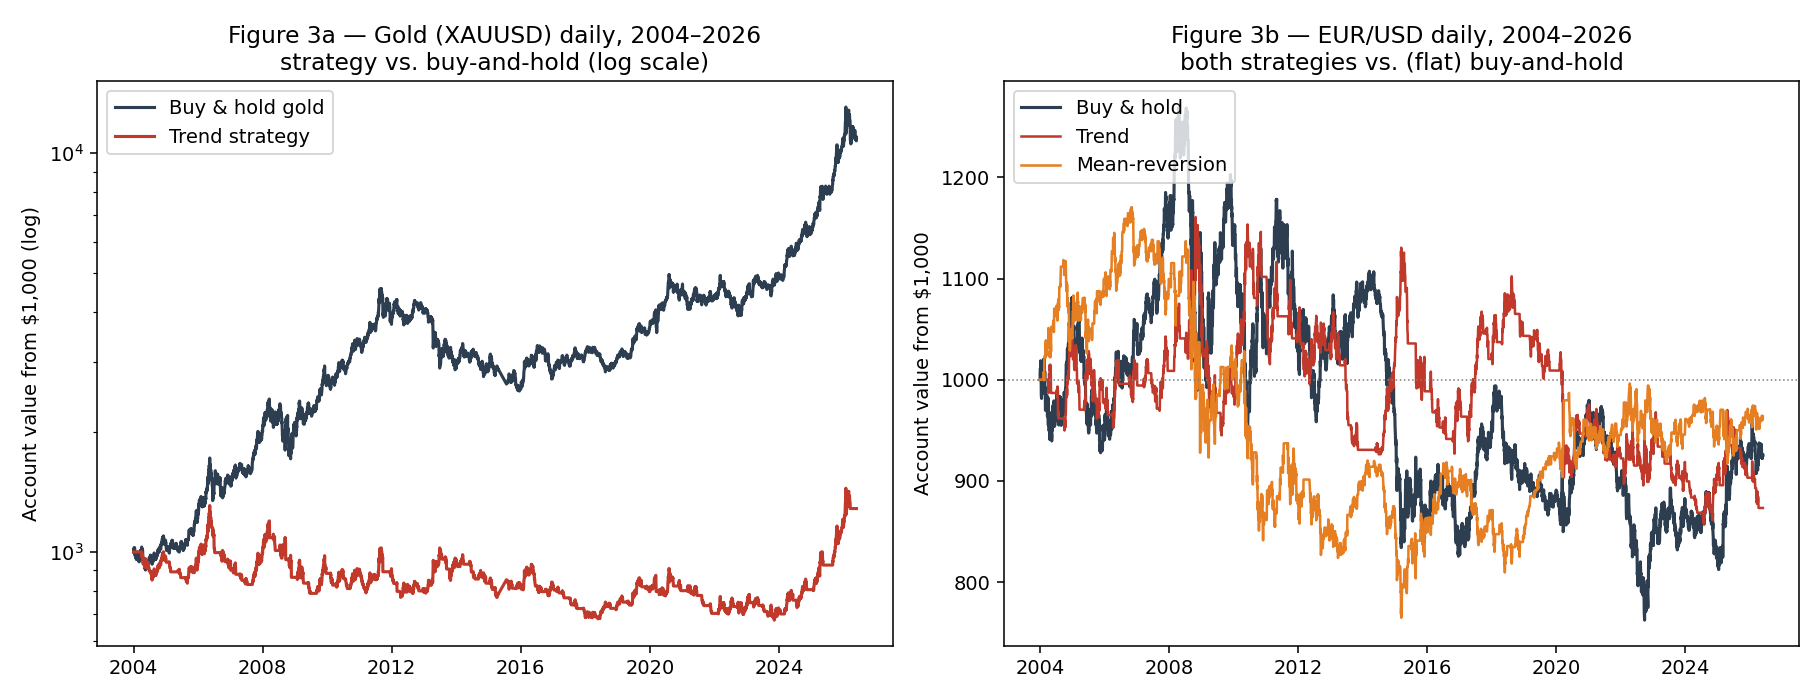
\includegraphics[width=\linewidth]{figures/fig3_equity_curves.png}
\caption{Left (gold, log scale): the trend strategy flatlines near its starting capital while buy-and-hold compounds $\sim$10$\times$. Gold enjoyed a once-in-a-generation bull market --- the ideal trend-following environment --- and the strategy still could not profit. Right (EUR/USD, linear): with a \emph{flat} benchmark, both strategies still drift below the \$1{,}000 line --- the cleaner disproof, showing negative expectancy on their own merits.}
\end{figure}

\subsection{Statistical significance}
A Sharpe of $S$ over $Y$ years implies a $t$-statistic of roughly $S \times \sqrt{Y}$. The two strongest results: gold-trend D1 $\to 0.18 \times \sqrt{22.4} \approx 0.85$; gold-trend H1 $\to 0.33 \times \sqrt{8.4} \approx 0.96$. Both are far below the $\approx 2.0$ threshold for significance --- meaning even the best returns are \textbf{indistinguishable from luck}, even with two decades of data.

\section{Forward (Paper) Testing}\label{sec:forward}
The paper engine was run live against the demo account (EUR/USD, mean-reversion, 15-minute bars, polling every 60\,s). Two findings:
\begin{enumerate}[leftmargin=1.6em]
  \item \textbf{Zero trades over several hours.} A 2$\sigma$ mean-reversion rule only fires when price closes outside the band ($\sim$5\% of bars); in a calm session it does not trigger. Equity stayed flat --- the strategy correctly waiting, not a fault.
  \item \textbf{A latent resilience bug, surfaced and fixed.} After $\sim$3\,h\,14\,m the loop crashed with \tbot{TimeoutError: (5, 'Deferred')}. Root cause: the SDK places a short timeout on each request's response \tbot{Deferred}, raising \tbot{twisted.internet.defer.TimeoutError} --- a class \emph{not} in the retry's transient list (neither an \tbot{OSError} nor a \tbot{crochet.TimeoutError}), so the retry never engaged and the exception tore down the loop. \textbf{Fix:} add the class to the transient list (with a regression test reproducing the exact exception), and wrap each loop tick so any single failure is logged and skipped rather than fatal. This is the value of forward-testing: a crash bug was found and fixed with \textbf{zero capital at risk}.
\end{enumerate}

\section{Discussion}
\textbf{Why no edge?} The results are consistent and, in aggregate, conclusive: simple technical rules do not yield a durable, tradeable edge on these liquid markets after costs. Three mechanisms explain it:
\begin{itemize}[leftmargin=1.4em]
  \item \textbf{Market efficiency.} EUR/USD and gold are among the most heavily-traded instruments on earth; any edge visible in public price history is competed away by faster, better-capitalised participants.
  \item \textbf{Buy-and-hold is a high bar.} For an appreciating asset (gold), the active strategy must beat $\sim$11\%/yr of ``do nothing.'' It captured $\sim$1\%/yr. Timing in and out mostly \emph{removed} return and \emph{added} drawdown.
  \item \textbf{Strategy/regime fit is real but not enough.} Mean-reversion (the correct tool for ranging FX) decisively beat trend-following on EUR/USD ($-$3.7\% vs $-$12.7\%, 65\% vs 32\% win rate) --- but ``better than the wrong tool'' still landed at breakeven-negative.
\end{itemize}

\noindent\textbf{Two cautionary lessons, observed directly:}
\begin{enumerate}[leftmargin=1.6em]
  \item \textbf{The small-sample mirage.} Gold-trend showed profit factor \textbf{1.80 on 38 trades} in an early study; on the full \textbf{639-trade} dataset it collapsed to \textbf{1.08}. An ``edge'' can be pure luck of a short window.
  \item \textbf{The regime bet masquerading as edge.} Mean-reversion on EUR/USD was \emph{positive} over the rangebound 2018--2026 window (+5.9\%) but \emph{negative} over the trend-containing 2004--2026 window ($-$3.7\%). Its apparent edge is a bet on a regime that nets to $\approx$ zero across a full cycle.
\end{enumerate}

\noindent\textbf{The honest conclusion on alpha.} The reliable improvements that remain are \emph{risk-adjusted}, not predictive: volatility targeting and diversification improve risk-adjusted return without forecasting direction. Trend-following's genuine (modest, eroding) premium lives at the diversified-portfolio level (managed-futures funds run it across 50--100 markets), not single-market and not at a size a \$1{,}000 account can implement. For an individual seeking to grow capital, the data's verdict is blunt: a low-cost, diversified buy-and-hold beats everything tested here.

\section{Limitations and Threats to Validity}
\begin{itemize}[leftmargin=1.4em]
  \item \textbf{In-sample only.} Backtests were not split into out-of-sample / walk-forward windows. This \emph{overstates} achievable performance --- yet every in-sample result already shows no edge, and out-of-sample can only be equal or worse, so the negative conclusion is \emph{robust} to this limitation.
  \item \textbf{Single data source.} All candles come from one broker's feed; pre-2015 daily data quality is unverified.
  \item \textbf{Optimistic costs.} The model excludes overnight swap/financing, which penalises multi-day trend positions and would push the marginal mean-reversion result (PF 1.02, 2{,}278 trades) further negative.
  \item \textbf{Demo execution.} Forward testing used a demo account; real fills, news-time slippage, and partial fills are not fully represented.
  \item \textbf{Limited instrument sweep.} Only gold and EUR/USD were backtested in depth; metals and indices were identified but not exhaustively tested.
  \item \textbf{Parameter risk.} Only a few parameter sets were tested, intentionally, to avoid data-dredging --- chasing the best-looking backtest across many configs is the principal route to overfitting.
\end{itemize}

\section{Future Work}
In priority order, none of which requires finding a ``magic'' strategy:
\begin{enumerate}[leftmargin=1.6em]
  \item \textbf{Walk-forward validation harness} --- tune on a rolling in-sample slice, score on a held-out out-of-sample slice. The rigour capstone.
  \item \textbf{Auto-reconnect on stale connection} --- so an unattended run self-heals (tracked as issue \#48).
  \item \textbf{Volatility-targeting overlay} --- the one reliable lever for improving risk-adjusted return without predictive edge.
  \item \textbf{A genuinely orthogonal input} --- e.g.\ trade gold only with the real-yield / dollar macro tide; most technical indicators are redundant transforms of price.
  \item \textbf{Diversified multi-market trend} --- the academically-supported form, requiring capital and breadth beyond the current account.
\end{enumerate}

\section{Conclusion}
The engineering objective was achieved completely: a safe, observable, broker-integrated, idempotent, well-tested (114 passing tests) trading system, built from first principles and exercised end-to-end against a live demo account. The trading objective was not achieved --- and the central contribution is to have demonstrated, rigorously and with two decades of data, \textbf{why}: simple technical strategies do not possess a durable, tradeable edge on these liquid markets after costs, and passive holding dominates. The clearest single statement of the result is that over 22 years, \emph{holding} gold turned \$1{,}000 into $\sim$\$10{,}800 while \emph{trading} it turned \$1{,}000 into $\sim$\$1{,}285, with a 48\% drawdown along the way.

This is not a failed project; it is a \emph{successful inquiry with a negative result} --- the kind most retail traders never reach, because they stop at one lucky backtest and convince themselves otherwise. The system stands as both a portfolio-grade engineering artifact and a piece of honest empirical evidence: in markets this efficient, the durable edge is not in the timing rules --- it is in bearing risk patiently, managing it well, and resisting the seduction of an overfit curve.

\appendix
\section{Technology Stack}
\begin{table}[ht]\centering
\begin{tabular}{@{}ll@{}}
\toprule
\textbf{Concern} & \textbf{Choice} \\
\midrule
Language / tooling & Python 3.12, \tbot{uv}, \tbot{ruff}, \tbot{pytest} (114 tests) \\
Data / storage & TimescaleDB (Postgres) $+$ Redis, via Docker Compose \\
DB access & SQLAlchemy 2.0 Core, psycopg 3 \\
Broker / API & FP Markets cTrader Open API, Twisted $+$ \tbot{crochet} \\
Config / logging & pydantic-settings, structlog \\
CLI & Typer $+$ Rich (\tbot{tbot}) \\
Backtesting & vectorbt 0.28.2 \\
\bottomrule
\end{tabular}
\end{table}

\section{Key CLI Commands}
\begin{verbatim}
tbot ctrader login                 # OAuth: obtain/refresh API tokens
tbot fetch XAUUSD D1 --since 2004-01-01
tbot backtest -s donchian -i XAUUSD -g D1 --entry-period 55 --exit-period 20
tbot backtest -s meanrev  -i EURUSD -g D1 --period 20 --num-std 2.0
tbot paper -s meanrev -i EURUSD -g M15 --loop   # demo-only forward test
tbot safety                        # confirm live orders are blocked
tbot status | reconcile | report   # observability
\end{verbatim}

\section{Reproducing the Figures}
\begin{verbatim}
uv run python docs/thesis/make_figures.py
\end{verbatim}
Bar charts (Figures~1--2) use the recorded scorecard; equity curves (Figure~3) are regenerated from stored candles via the project's own \texttt{run\_backtest}.

\section{Safety Posture (unchanged throughout)}
\tbot{ALLOW\_LIVE\_TRADING=false} and \tbot{CTRADER\_ENV=demo} for the entirety of this work. No live order was ever placed; the live account was used only for read-only data and demo execution.

\end{document}
